% Created 2020-06-24 Wed 17:12
% Intended LaTeX compiler: pdflatex
\documentclass[bigger]{beamer}
\usepackage[utf8]{inputenc}
\usepackage[T1]{fontenc}
\usepackage{graphicx}
\usepackage{grffile}
\usepackage{longtable}
\usepackage{wrapfig}
\usepackage{rotating}
\usepackage[normalem]{ulem}
\usepackage{amsmath}
\usepackage{textcomp}
\usepackage{amssymb}
\usepackage{capt-of}
\usepackage{lmodern}
\usepackage{hyperref}
\usepackage{kky}
\usepackage{multimedia}
\newcommand{\video}[1]{ \movie[poster, height = 0.8\textheight, width = \textwidth, autostart, loop, poster]{}{#1}}
\usetheme{Madrid}
\author[Hugo Richard \emph{et al.}]{Hugo Richard, Pierre Ablin,  Alexandre Gramfort, Bertrand Thirion, Aapo Hyvarinen}
\date{NeurIPS, 2021}
\title[ShICA]{Shared Independent Component Analysis for Multi-Subject Neuroimaging}
\titlegraphic{
  Github: @hugorichard $\begin{array}{l}
                                      
\includegraphics[width=1cm]{github.png}
                                    \end{array}$
                                     \hspace*{0.1\textwidth}~%
                                     Twitter: @hugorichard $\begin{array}{l}
                                                              
\includegraphics[width=1cm]{twitter.png}
                                                            \end{array}$ \\
                                                            \color{blue}{\url{https://hugorichard.github.io}}

                                                             $\begin{array}{l}
                                                                
\includegraphics[height=1cm]{inria.png} \end{array}$
                                                              $\begin{array}{l} 
\includegraphics[height=1cm]{ups.png} \end{array}$
                                                              \\

                                                          }
\setbeamertemplate{navigation symbols}{}
\begin{document}

\maketitle

\section{Introduction}
\label{sec:orgea2ebd0}
\begin{frame}[label={sec:org0e5a650}]{Sources and sensors}
\video{source_emission.mp4}
\end{frame}
\begin{frame}[label={sec:orgc5c8b11}]{Mixing}
\video{source_mixing.mp4}
\end{frame}
\begin{frame}[label={sec:org3d37d88}]{Independent component analysis (noise-free)}
\begin{block}<1->{ICA model (Jutten, 1991)}
\begin{itemize}
\item Independent \emph{sources}: \(\sbb \in \mathbb{R}^{k}\)
\end{itemize}
\(p(\sbb) = p(s_1) \cdots p(s_k)\)
\begin{itemize}
\item \emph{\emph{Sensors}}: \(\xb \in \mathbb{R}^{k}\)
\end{itemize}

\centering
\emph{\emph{\(\xb = A\sbb\)}}

where \(A\) is the \emph{Mixing matrix}. 
\end{block}

\only<2>{
  $\begin{matrix} 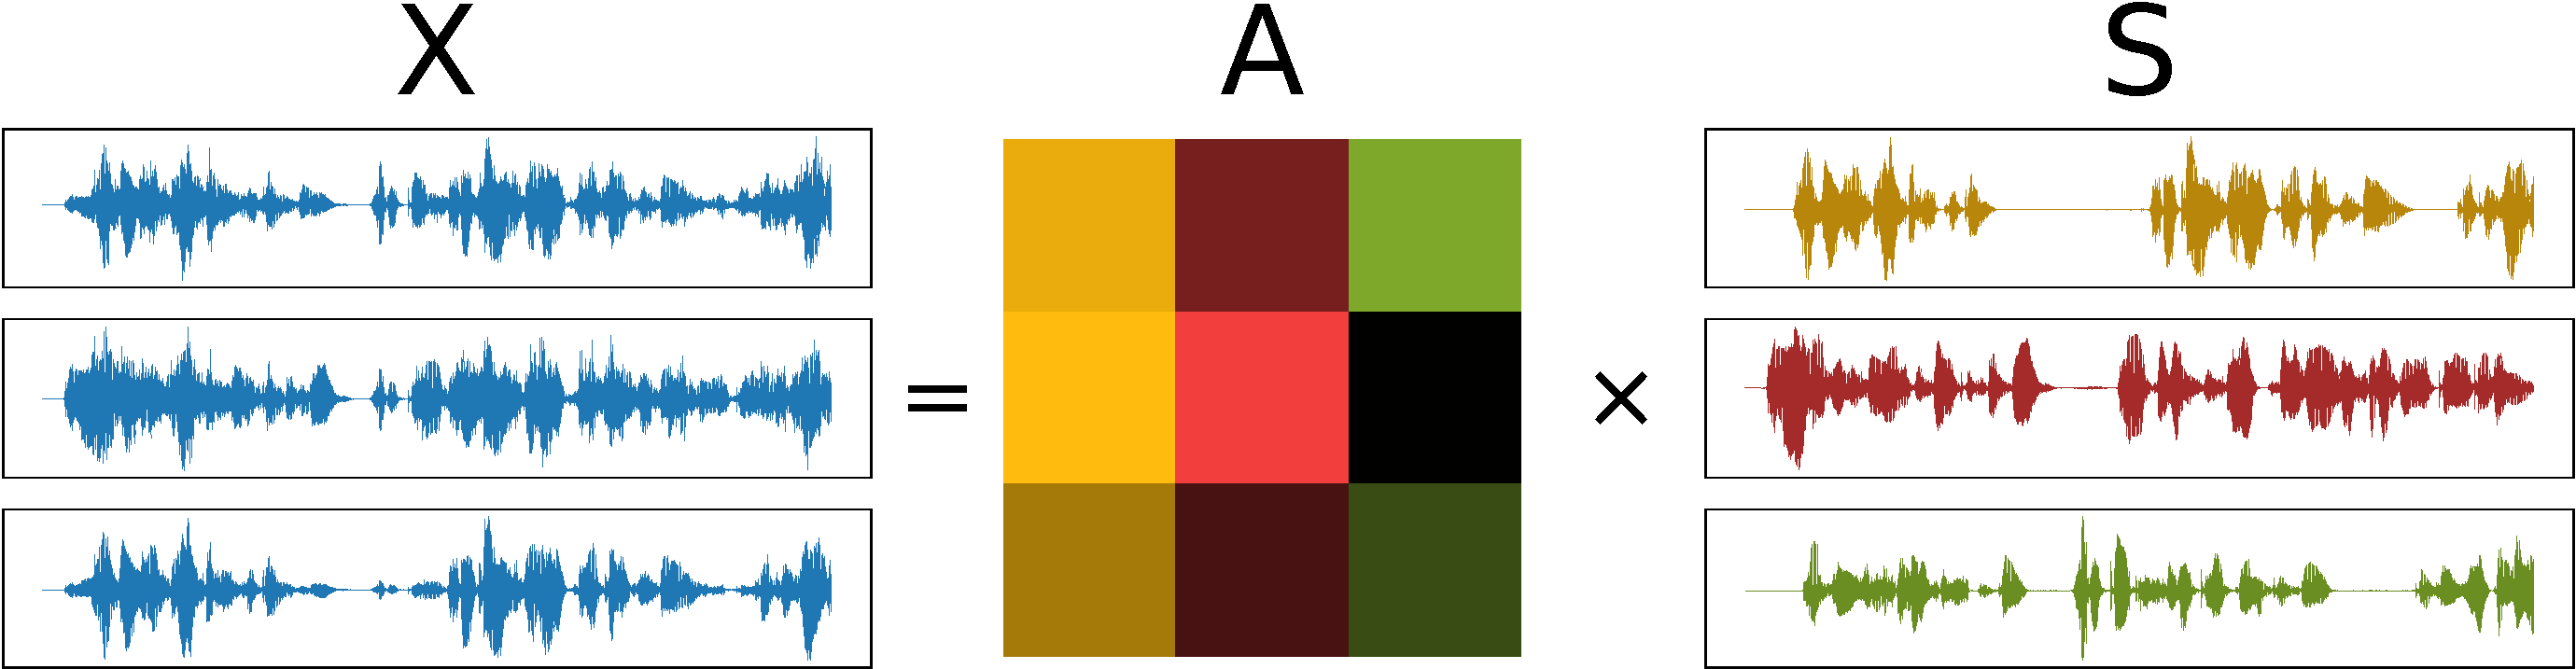
\includegraphics[width=6.2cm]{indet_1.pdf} \end{matrix}$ \hspace{0.5cm} $\begin{matrix} 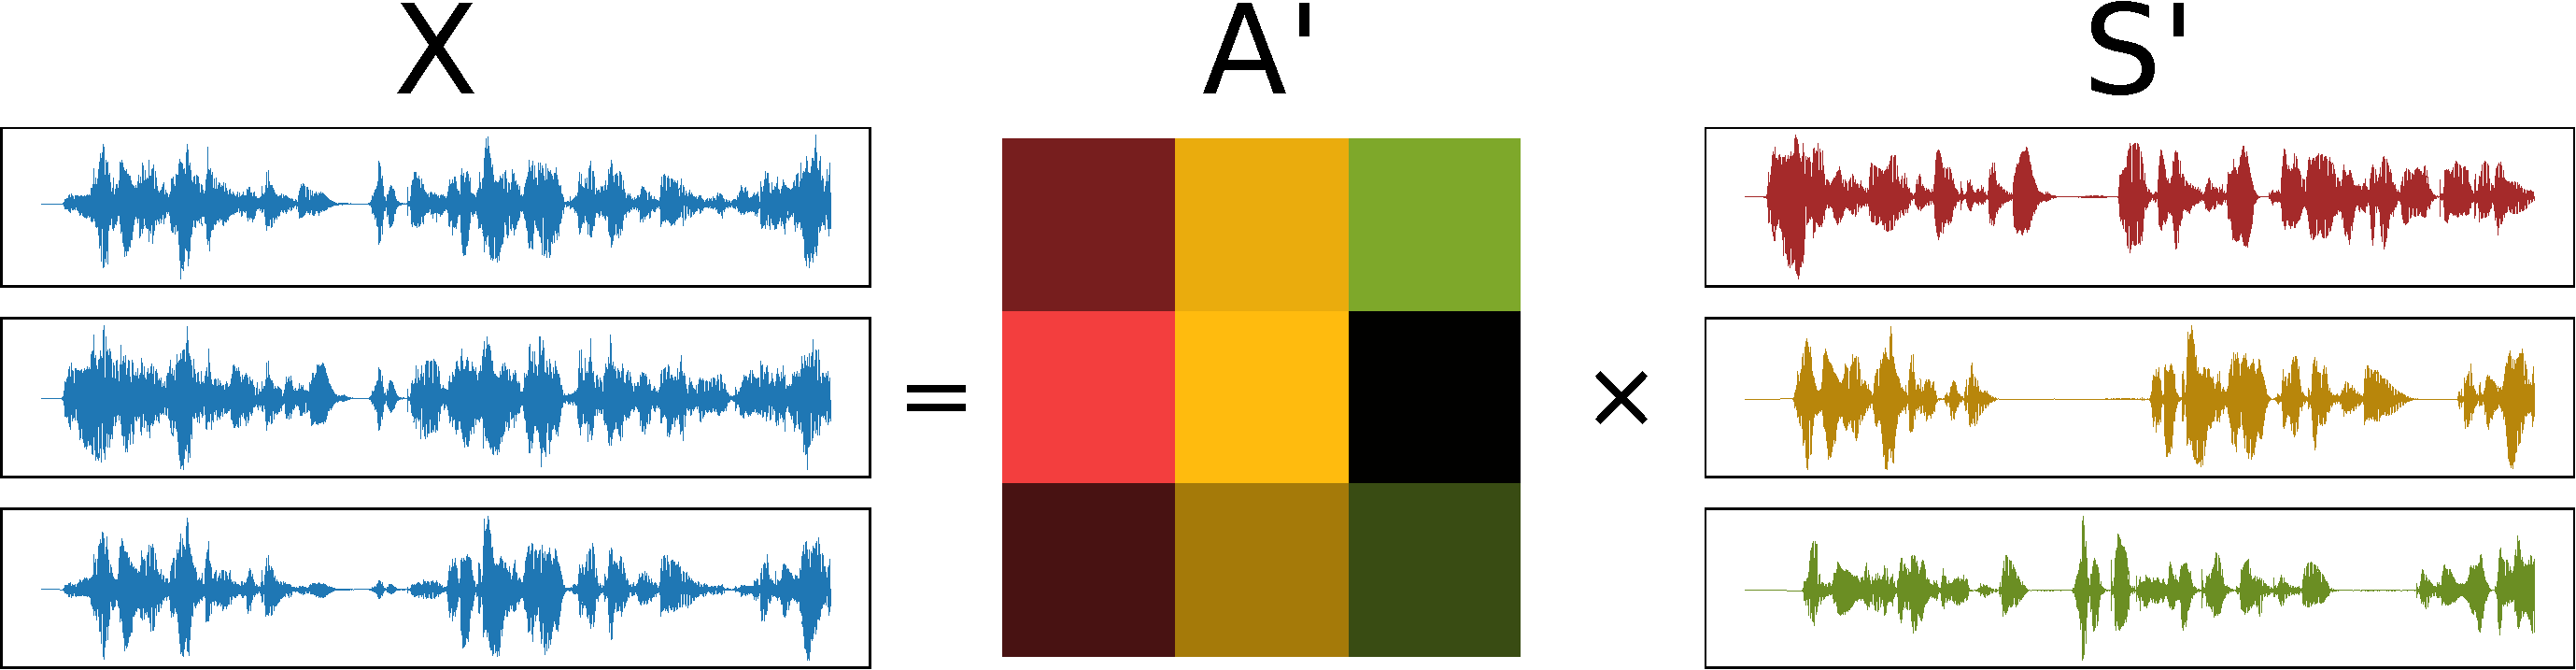
\includegraphics[width=5cm]{indet_2.pdf}\\  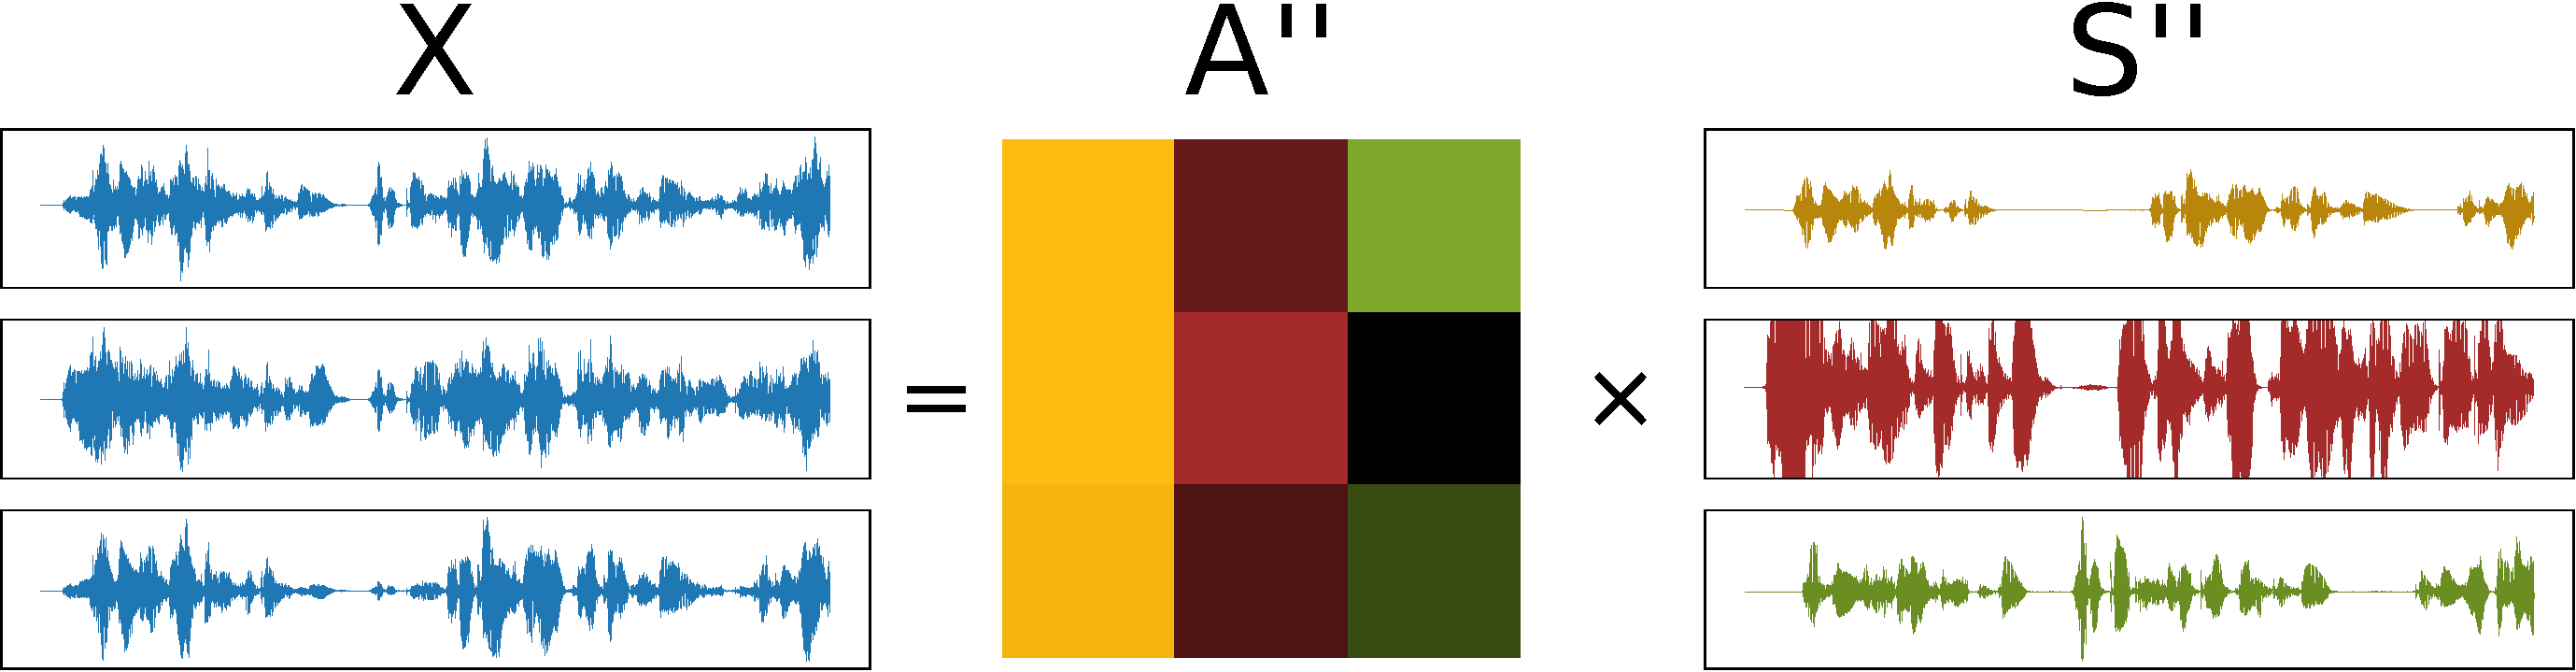
\includegraphics[width=5cm]{indet_3.pdf}\end{matrix}$
}
\begin{theorem}<3->[Identifiability of ICA (Common, 1994)]
  If \(\xb = A \sbb\) and \(\xb = A' \sbb'\)
  and if $\sbb$ has at most one Gaussian component,

Then 
\begin{itemize}
\item \(A = P A'\)
\item \(P\) is a scale and permutation matrix.
\end{itemize}
\end{theorem}
\end{frame}

\section{Group ICA}
\label{sec:orgde83014}
\begin{frame}{Group ICA}
\begin{block}{Generalization to multiple subjects exposed to the same stimuli}
  Consider 2 subjects \(\xb_1, \xb_2 \in \mathbb{R}^k\) such that
  \begin{itemize}
  \item $\xb_1 = A_1 \sbb + \nb_1$
  \item $\xb_2 = A_2 \sbb + \nb_2$
  \end{itemize}
\end{block}
\begin{block}{Interpretation}
  \begin{itemize}
  \item Shared sources $\sbb$: shared cognitive processes 
  \item Different mixing matrices $A_i$: different spatial topography of each subject
  \item Different noises $\nb_i$: inter-subject variability.
  \end{itemize}
\end{block}
\end{frame}

\begin{frame}{State of the art}
\begin{block}{ConcatICA [Calhoun, 2001]}
  \(\xb_1 \in \mathbb{R}^{k}, \xb_2 \in \mathbb{R}^{k}\)
  \begin{itemize}
  \item PCA of \(\xb = \begin{bmatrix} \xb_1 \\ \xb_2 \end{bmatrix}\)
  \end{itemize}
  \(\xb = \begin{bmatrix} U_1 \\ U_2 \end{bmatrix}  \xb_{red} \), 
  where \( \xb_{red}  \in \mathbb{R}^{k}\) and 
  \(\begin{bmatrix} U_1 \\ U_2 \end{bmatrix}\)
  is orthogonal.
  \begin{itemize}
  \item ICA of reduced data \( \xb_{red}  = A \sbb\)
  \end{itemize}
\end{block}
\begin{block}{CanICA [Varoquaux, 2010]}
  Replace PCA with (multi-set) CCA in ConcatICA \\
  CCA solves:
  $\begin{bmatrix} \EE[\xb_1 \xb_1^{\top}] & \EE[\xb_1 \xb_2^{\top}] \\
    \EE[\xb_2 \xb_1^{\top}] & \EE[\xb_2 \xb_2^{\top}]\end{bmatrix} \begin{bmatrix}
    \ub_1 \\ \ub_2 \end{bmatrix} =
  \lambda \begin{bmatrix} \EE[\xb_1 \xb_1^{\top}] & 0 \\
    0 & \EE[\xb_2 \xb_2^{\top}]\end{bmatrix} \begin{bmatrix}
    \ub_1 \\ \ub_2 \end{bmatrix}$
\end{block}
\end{frame}

\begin{frame}{State of the art}
  \begin{block}{About CanICA and ConcatICA}
    \begin{itemize}
    \item Very fast to fit
    \item Simple to implement
    \item Do not optimize a proper likelihood
    \item Not even clear what is the underlying model
    \end{itemize}
  \end{block}

  \begin{block}{Some other related work}
    \begin{itemize}
    \item IVA [Lee, 2008] 
    \item Unified approach [Guo, 2008] 
    \item SRM [Chen, 2015] 
      \item MultiViewICA [Richard, 2020]
    \end{itemize}
  \end{block}
\end{frame}


\section{Exact likelihood}
\label{sec:org55f3e63}
\begin{frame}{Noisy ICA}
\begin{example}[Noisy ICA likelihood with Gaussian mixtures (Bermond, Cardoso, 1999)]
  \underline{Our model}:
\begin{itemize}
\item $\xb_i = A_i \sbb + \nb_i, \nb_i \sim N(0, \sigma^2 I_{k})$
  $I_{k} \in \mathbb{R}^{k, k}$ is the identity matrix.
\item $p(s_j) = \frac1{q} \sum_{\alpha_j \in \mathcal{A}} \mathcal{N}( s_j; 0,
  \alpha_j)$,  $\mathcal{A} \in (\RR^*_+)^q$\\
\end{itemize}

\underline{Solving via EM}\\
E-step: \\
\begin{itemize}
\item $p(\sbb | \xb) = \sum_{\alphab, \alpha_j \in \mathcal{A}} p(\sbb | \xb,
  \alphab) p(\alphab | \xb)$, with $\xb = \xb_1,  \cdots, \xb_n$ and $\alphab =
  \alpha_1, \cdots, \alpha_k$
\end{itemize}

  But \underline{$\{\alphab, \alpha_j \in \mathcal{A}\}$ has size $q^k$} making the E-step intractable.
\end{example}
\end{frame}

% \section{Optimization}
% \label{sec:org6a44715}
% \begin{frame}[label={sec:orgee78096}]{Optimization}
% \begin{block}{Fast optimization}
% \begin{itemize}
% \item Alternate optimization (alternate between subjects)
% \item Quasi newton with an approximation of the Hessian
% \end{itemize}
% \end{block}
% \begin{block}{Quasi-Newton}
% \begin{itemize}
% \item Updates \(W_i = (I + \rho D)W_i\), \(D = {H_i}^{-1} G_i\) such that
% \end{itemize}
% \(\mathcal{L}((I + \varepsilon)W_i)) = \mathcal{L}(W_i) + <\varepsilon | G_i> +
% <\varepsilon | H_i \varepsilon>, \enspace H_i \in \mathbb{R}^{k \times k \times k \times k}\)
% \begin{align}
%   \label{eq:hessian}
%   \only<1>{(\mathcal{H}_i)_{abcd} &= \delta_{ad}\delta_{bc} + \delta_{ac}\left(\frac{1}{m^2}f''(\tilde{s}_a) + \frac{1 - 1/m}{\sigma^2}\right)y_{ib}y_{id} \\ & \text{where} \enspace \yb_i = W_i \xb_i}
%                                                                                                                                                                 \only<2>{(H_i)_{abcd} &= \delta_{ad}\delta_{bc} + \delta_{ac}\delta_{bd}\left(\frac{1}{m^2}f''(\tilde{s}_a) + \frac{1 - 1/m}{\sigma^2}\right)\left(y_{ib}\right)^2 \\ & \text{where} \enspace \yb_i = W_i \xb_i}
% \end{align}
% \only<1>{$\mathcal{H}_i$ has $O(k^3)$ non zero coefficients.}
% \only<2>{$H_i$ has $O(k^2)$ non zero coefficients. It is 2x2 block
%   diagonal: easy to invert and regularize}
% \end{block}
% \end{frame}


\begin{frame}{Our contribution: Shared ICA (ShICA)}
  \begin{block}{ShICA model}
     \begin{center}$ \xb_i = A_i (\sbb + \nb_i), i=1,\dots, m$ \end{center}
    \begin{itemize}
      \item $\nb_i \sim \Ncal(0, \Sigma_i)$ where $\Sigma_i$ is diagonal positive.
      \item $\sbb$ are independent components some of which may be Gaussian
      \item $\EE[\xb_i] = 0$, $A_i$ invertible, $\EE[\sbb \sbb^{\top}] = I_k$ and $m \geq 3$
     \end{itemize}
  \end{block}
  \begin{block}{ShICA-J: }
    \begin{itemize}
\item In theory Multiset CCA solves ShICA (under some conditions).
\item In practice, sampling noise causes some issues.
\item Joint diagonalization solves it: ShICA-J = MCCA + Joint diag
  \end{itemize}
  \end{block}
  \begin{block}{ShICA-ML}

    \begin{itemize}
  \item A maximum likelihood approach to ShICA
    \end{itemize}
  \end{block}
\end{frame}

\begin{frame}{ShICA is identifiable}
  \begin{definition}[Noise diversity in Gaussian components]
    Let $\mathcal{G}$ be the set of Gaussian components. For all $j, j'  \in \mathcal{G}, j \neq j'$, the sequences $(\Sigma_{ij})_{i=1 \dots m}$ and $(\Sigma_{ij'})_{i=1 \dots m}$ are different where $\Sigma_{ij}$ is the $j, j$ entry of $\Sigma_i$.
  \end{definition}
\begin{theorem}[Identifiability]
  Assuming noise diversity, let $\Theta=(A_1, \dots, A_m, \Sigma_1, \dots,\Sigma_m)$ be the set of
  parameter that generates $\xb_1 ,\dots, \xb_m$ from the ShICA model. 
  We let $\Theta'=(A_1', \dots, A_m', \Sigma_1', \dots,\Sigma_m')$ another set
  of parameters, and assume that they also generate the data. Then, there exists a sign and permutation matrix $P$ such that for all $i$, $A_i'=A_iP$, and $\Sigma_i'= P^{\top} \Sigma_i P$.
\end{theorem}
Note that noise diversity in Gaussian component is also a necessary condition.
\end{frame}

\begin{frame}{Multiset CCA solves GroupICA}
  \begin{theorem}[Solving GroupICA with Multiset CCA]
    We assume $\xb_i$ follows $\xb_i = A_i (\sbb + \nb_i)$ where  $\nb_i \sim \Ncal(0, \Sigma_i)$ where $\Sigma_i$ is diagonal and consider the multiset CCA
    problem \\
      $C \ub = \lambda D \ub$ \\
      where block $i, j$ of $C$ is $\EE[\xb_i \xb_j^{\top}]$ and $D$ is block
      diagonal with block $i, i$ given by $\EE[\xb_i \xb_i^{\top}]$.
      Let $U = [\ub_1 \dots \ub_k] = \begin{bmatrix} W_1^{\top} \\ \vdots \\
        W_m^{\top} \end{bmatrix}$ where $W_i \in \RR^{k, k}$.  \\
      Then \underline{if $\lambda_1 \dots \lambda_k$ are distincts}, $W_i = P \Gamma_i A_i^{-1}$ where $P$ is a permutation matrix and
      $\Gamma_i$ a scaling matrix.  
  \end{theorem}
  Note that the distinct eigenvalue condition is also necessary.

  Note that the condition is stronger than noise diversity (we can exhibit an identifiable
  example on which MCCA fails).
\end{frame}

\begin{frame}{Practical issues with Multiset CCA}
    The mapping from matrices to eigenvectors is
    highly non smooth...
  \begin{block}{Practical example}
    $m=3$, $k=2$ and $\Sigma_i$ such that $\lambda_1 = 2 + \epsilon$ and $\lambda_2
    = 2$. \\
    $W_i$: Solution of multiset CCA on true covariance matrices $C_{ij}$ \\
    $\tilde{W}_i$: Solution of multiset CCA on perturbed covariance matrices 
    $\tilde{C}_{ij} = C_{ij} + \delta S$ where $S$ positive
    symmetric matrix of norm $1$.
  \end{block}
  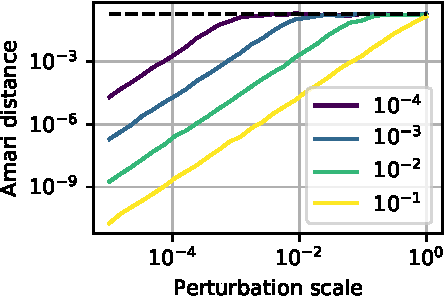
\includegraphics[scale=0.8]{figures/multicca_gap.pdf}
\end{frame}

\begin{frame}{Solving practical issues with joint diagonalization}
  \begin{block}{Large gap between the first $k$ eigenvalues and others}
    $\lambda_k - \lambda_{k+1} > \frac{m-1}{1 + \max_{ij} \Sigma_{ij}} +
    \frac1{1 + \min_{ij} \Sigma_{ij}}$
  \end{block}
  \begin{block}{Practical implications}
    The span of the $p$ leading eigenvectors is preserved:
    $W_i \approx Q \tilde{W}_i$.
    We recover $Q$ by joint diagonalization of $Q \tilde{W}_i \frac1{n}X_i X_i^{\top} \tilde{W}_i^{\top}Q^{\top}$
  \end{block}
  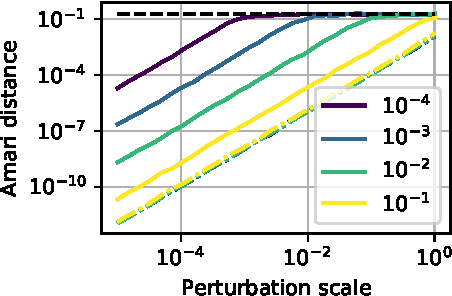
\includegraphics[scale=0.8]{figures/multicca_gap_jd.pdf}
\end{frame}

\begin{frame}{ShICA-J}
 Use Multiset CCA and joint diagonalization to obtain $W_i$ up to a
    scaling $\Psi_i$.
  \begin{block}{Find the scalings}
    We solve $\min_{\Psi} \sum_{i \neq j} \|\Psi_i \diag(Q \tilde{W}_i
    \tilde{C}_{ij} \tilde{W}_j Q^{\top}) \Psi_j - I_k \|^2$.
    The estimates of $W_i$ are then given by $\hat{W}_i = \Psi_i Q \tilde{W}_i$.
  \end{block}

  \begin{block}{Find the noise variances}
    We use the maximum likelihood estimate of $\xb_i = \hat{W}_i^{-1}(\sbb +
    \nb_i)$ via an EM algorithm.
    The E-step and M-step are in closed form yielding a fast algorithm.
  \end{block}
  ShICA-J is very fast. But it is not a maximum likelihood estimator.
\end{frame}


\begin{frame}{ShICA-ML: the maximum likelihood estimator}
  \begin{block}{ShICA-ML}
      \centerline{$\xb_i = A_i (\sbb + \nb_i)$} where $\nb_i \sim \Ncal(0, \Sigma_i)$, $\Sigma_i$ diagonal and $s_j
  \sim \frac12 \sum_{\alpha \in \{ \frac12, \frac32 \}} \Ncal(0, \alpha)$.
  \end{block}

  \begin{block}{Optimization}
    Optimized via an EM algorithm.
    \vspace{-1em}
    \begin{center}
      $\EE[s_j | \xb] = \frac{\sum_{\alpha \in \{\frac12, \frac32\}}
        \theta_{\alpha} \frac{\alpha \bar{y}_{j}}{\alpha +
          \bar{\Sigma_{j}}}}{\sum_{\alpha \in \{ \frac12, \frac32 \}}
        \theta_{\alpha}} $, $\enspace \enspace \enspace$
      $ \VV[s_j | \xb] = \frac{\sum_{\alpha \in \{\frac12, \frac32\}} \theta_{\alpha} \frac{\bar{\Sigma_{j}}\alpha}{\alpha + \bar{\Sigma_{j}}}}{\sum_{\alpha \in \{ \frac12, \frac32 \}} \theta_{\alpha}}$  
    \end{center}
    \vspace{-1em}
    where $\theta_{\alpha} = \Ncal(\bar{y}_{j}; 0 , \bar{\Sigma}_{j} + \alpha)$, 
    $\bar{y}_j = \frac{\sum_i \Sigma_{ij}^{-1} y_{ij}}{ \sum_i
      \Sigma_{ij}^{-1}}$ and $\bar{\Sigma_{j}} = (\sum_i
    \Sigma_{ij}^{-1})^{-1}$ with $\yb_i = W_i \xb_i$.
    M-step: Closed form updates for noise variances and quasi-newton updates for
    unmixing matrices.
  \end{block}
  ShICA-J provides a great initialization to ShICA-ML
\end{frame}

\begin{frame}{Synthetic experiments}
  \begin{block}{Separation performance depending on the density of sources}
  $m=4$ views, $k=5$ components, non-Gaussian sources are from a Laplace
  density, we use the ShICA model using: \\
  (a) Gaussian components with noise diversity \\
  (b) non-Gaussian components without noise diveristy \\
  (c) Half of components are Gaussian with noise diversity, the other half is
  non-Gaussian without diversity
\end{block}
  \begin{center}
    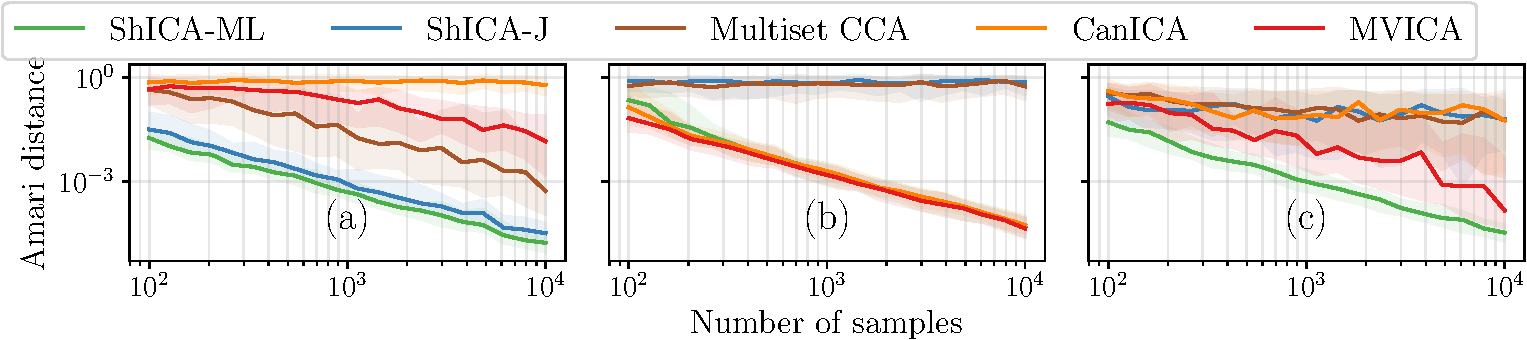
\includegraphics[width=\textwidth]{./figures/identifiability.pdf}
  \end{center}
\end{frame}

\begin{frame}{Synthetic experiments}
  \begin{block}{Computation time}
    We generate components from a slightly super-Gaussian density $s_j = d(x)$
    with $d(x) = x |x|^{0.2}$ and $x \sim \mathcal{N}(0, 1)$ vary the number of
    samples $n=10^2 \dots 10^4$.
  \end{block}
  \begin{center}
    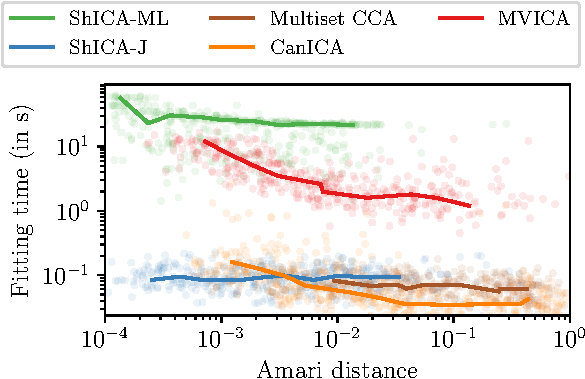
\includegraphics[width=0.65\textwidth]{./figures/synthetic_gaussian_timings.pdf}
  \end{center}
\end{frame}

\begin{frame}{Reconstruction experiment fMRI}

  \begin{columns}[T] % align columns
    \begin{column}{.4\textwidth}
      \begin{itemize}
      \item Train data: 100\% subjects 80\% runs -> Learn unmixing matrices
      \item Test data: 80\% subjects 20\% runs -> Compute sources
      \item Validation data: 20\% subjects 20\% runs -> Measure R2 score
      \end{itemize}
    \end{column}%
    \hfill%
    \begin{column}{.6\textwidth}
      \begin{center}
        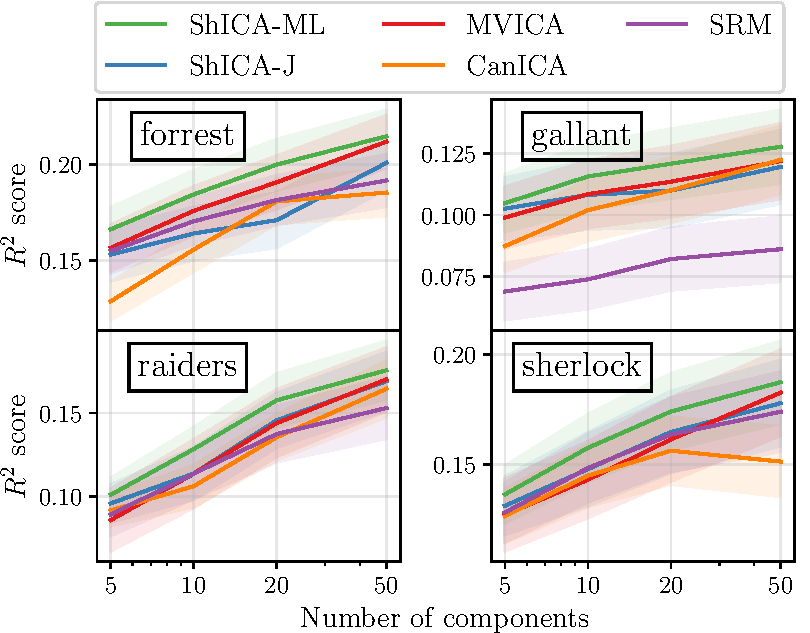
\includegraphics[width=\linewidth]{./figures/reconstruction.pdf}
      \end{center}
    \end{column}%
  \end{columns}
\end{frame}

\begin{frame}{Timesegment matching fMRI}
  \begin{columns}[T] % align columns
    \begin{column}{.4\textwidth}
      \begin{itemize}
      \item Timesegment matching accuracy: Locate a 9 timeframes timesegment in a left out subject by correlation with the average response of other subjects.
      \item Train data: 80\% runs $\rightarrow$ Learn unmixing matrices
      \item Test data: 20\% runs $\rightarrow$ Measure accuracy
      \end{itemize}
    \end{column}%
    \hfill%
    \begin{column}{.6\textwidth}

      \begin{center}
        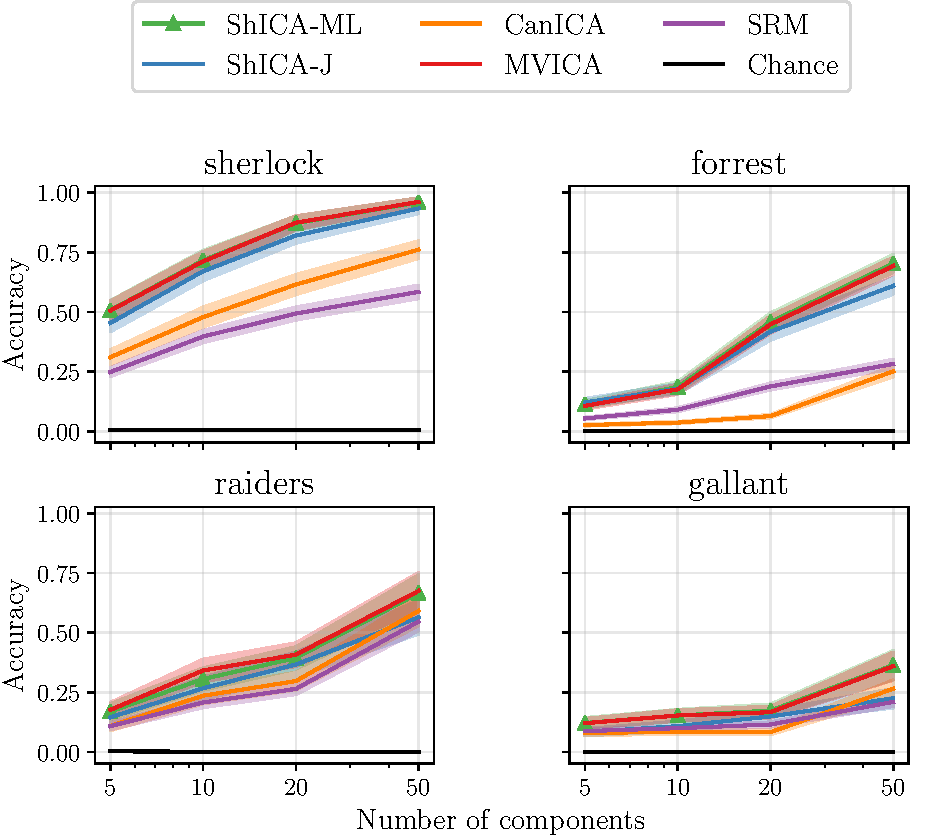
\includegraphics[width=\linewidth]{./figures/timesegment_matching.pdf}
      \end{center}
    \end{column}%
  \end{columns}
\end{frame}


\begin{frame}
  \begin{block}{MEG Phantom experiment}
    \begin{itemize}
    \item 8 dipoles in a plastic head at different locations
    \item Dipoles separately emit the same known signal $S_{true}$ during $n$ epochs
    \item $20$ sources estimated: the best one is compared with $S_{true}$
    \end{itemize}
  \end{block}
  \begin{center}
    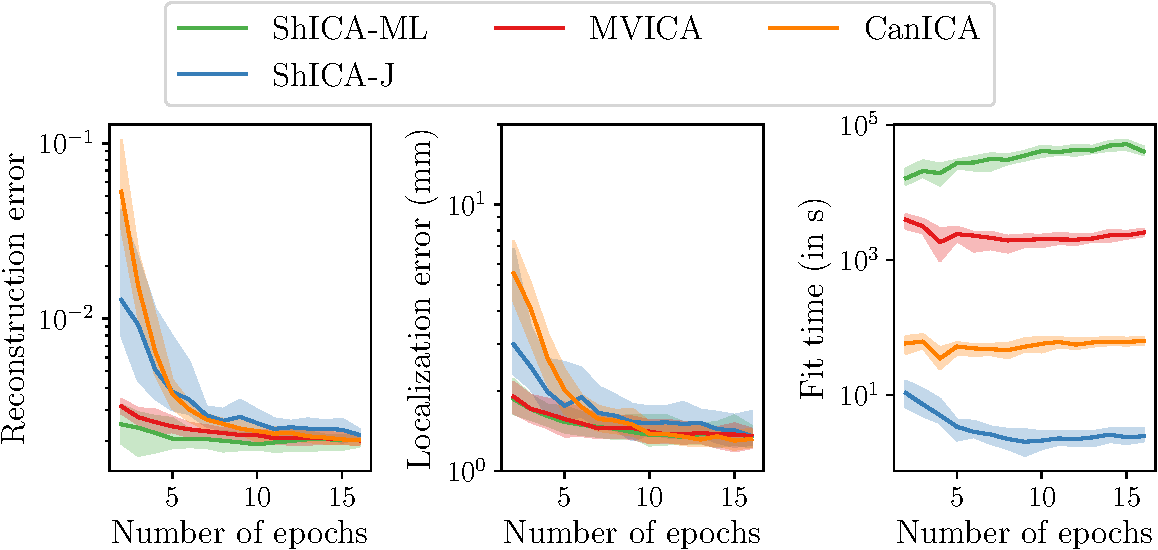
\includegraphics[width=0.7\textwidth]{./figures/meg_phantom_neurips.pdf}
  \end{center}
\end{frame}

\begin{frame}{Conclusion}
\begin{block}{Take home message}
\begin{itemize}
\item ShICA is a powerful framework to extract shared sources
\item ShICA-J yields a fast approach but only uses second order information,
  ShICA-ML is a bit slower but uses in addition non-Gaussianity.
\item Yields better results in practice: extensive comparison on multiple
  neuroscience modalities.
\end{itemize}
\end{block}

\begin{block}{Future Work}
\begin{itemize}
  \item These methods work on reduced data. How to provide the best dimension
    reduction method ?
  \item The non-Gaussian density of the shared sources in ShICA-ML could be learned.  
\end{itemize}
\end{block}
\end{frame}
\end{document}